\section{Obtain Image Segmentation by Active Contour Models}

Active Contour Models (also called ``snakes'') depend on adequately set parameters in order to work as desired. In this section we observed the effect of changing the parameters' values when trying to segment the outline of a heart from an image.

\subsection{Parameter Experiments}

The parameters to evaluate are the following:

\begin{itemize}

	\item $\alpha$: Controls the \textit{elasticity} of the model, with higher values corresponding to less stretching. A high $\alpha$ leads to the model trying to keep the points as close to each other as possible.
	
	\item $\beta$: Controls the \textit{rigidity} of the model, with higher values corresponding to less flexibility. A high $\beta$ leads to a model with as little curves as possible.
	
	\item $\lambda$: Controls the proportion of the balloon force. The model expands for $\lambda > 0$ and contracts for $\lambda < 0$.
	
	\item $\kappa$: Controls the proportion of the external force that stops the model when arriving at edges. High values of $\kappa$ make the model stop at weaker edges. In our case we set $ \kappa $ to $ \frac{\kappa'}{\max (G_x, G_y)} $, being $ G_x $ and $ G_y $ the components of the force field. We tweak $ \kappa' $ instead of $ \kappa $ itself.
	
	\item $maxstep$: Defines the maximum step size in pixel, aimed at minimizing unwanted crossing-over.
	
\end{itemize}

In the following we examine the effects of changing the value of the different parameters. We try to examine optimal and critical values. We keep a base configuration set of $(\alpha , \beta , \lambda , \kappa' , maxstep) = (0.1 , 0.01 , 0.05 , 0.2 , 0.4)$ and then change individual parameter values while keeping the others invariant.

\subsubsection{Alpha}

The parameter $\alpha$ controls the elasticity of the model. The given value of $0.1$ yields relatively good results. As can be seen in figure \ref{fig:alpha_leq},  our experiments showed that decreasing $\alpha$ to $0.05$ augments the results slightly, since the model can ``grow'' more tightly into the corners of the heart. When decreasing the value further, the model fails to stop at the edge of the heart segment and grows too far. The optimal value is thus somewhere near $0.05$ and the first critical value that leads to failure lies between $0.02$ and $0.05$.
\begin{figure}[!hbt]
\centering   
\subfigure[$\alpha=0.02$]{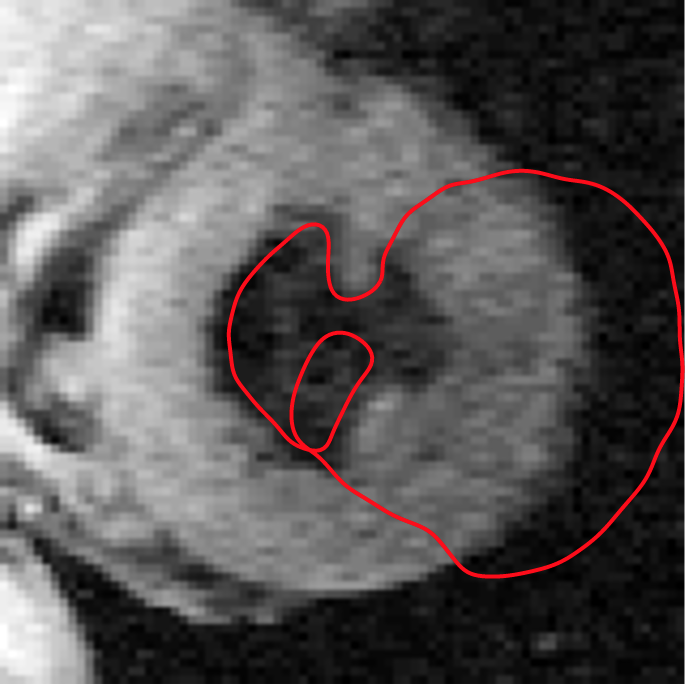
\includegraphics[width=40mm]{img/a0_02}}
\subfigure[$\alpha=0.05$]{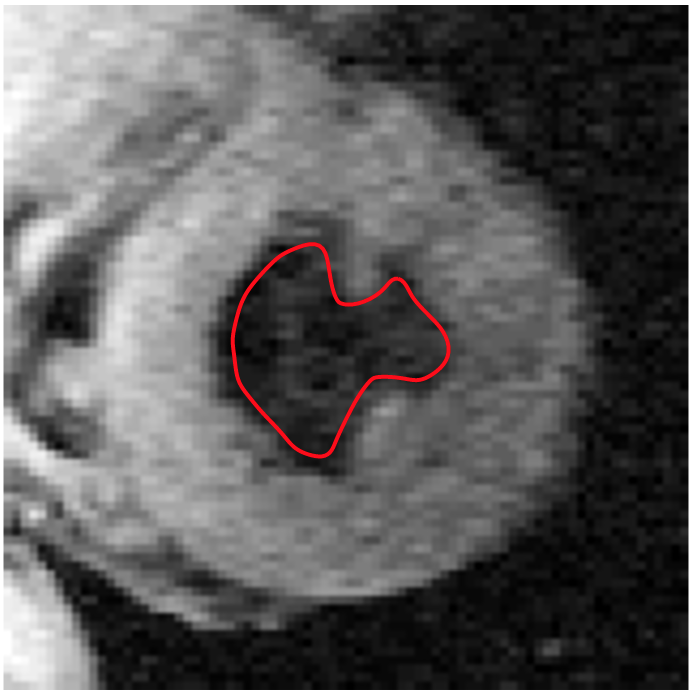
\includegraphics[width=40mm]{img/a0_05}}
\subfigure[$\alpha=0.1$]{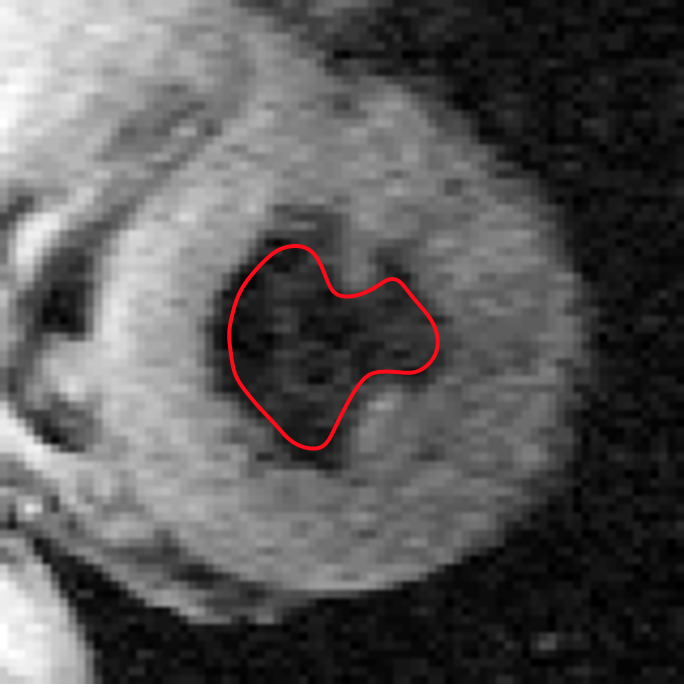
\includegraphics[width=40mm]{img/a0_1}}
\caption{Heart: tweaking the values of $ \alpha $. $\alpha \leq 0.1$}
\label{fig:alpha_leq}
\end{figure}

Our experiments show almost no change when increasing $\alpha$ to $0.15$. A value of $0.2$ already seems to be a critical value - the model does not expand at all and stops in the initial shape of a circle, see figure \ref{fig:alpha_geq}.

\begin{figure}[!hbt]
\centering   
\subfigure[$\alpha=0.1$]{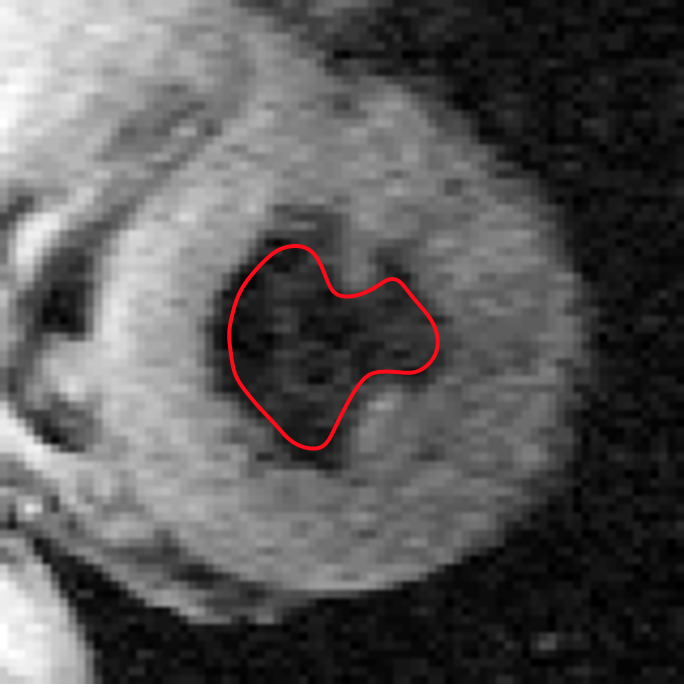
\includegraphics[width=40mm]{img/a0_1}}
\subfigure[$\alpha=0.15$]{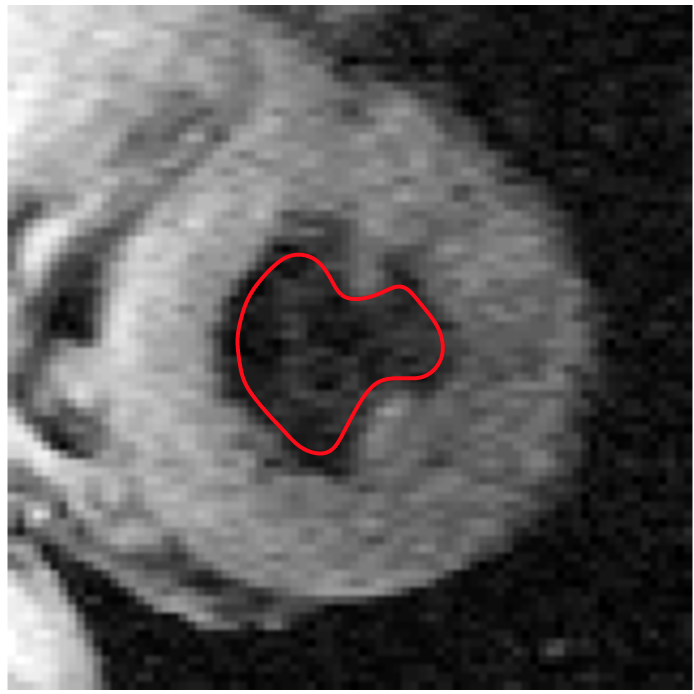
\includegraphics[width=40mm]{img/a0_15}}
\subfigure[$\alpha=0.2$]{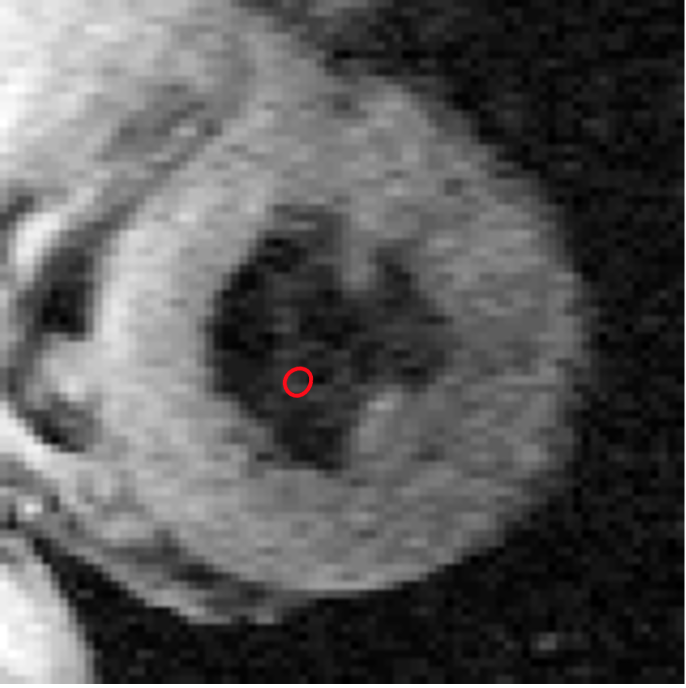
\includegraphics[width=40mm]{img/a0_2}}
\caption{Heart: tweaking the values of $ \alpha $. $\alpha \geq 0.1$}
\label{fig:alpha_geq}
\end{figure}

\subsubsection{Beta}

The parameter $\beta$ controls the rigidity of the model. As figure \ref{fig:beta_leq} shows, the initial value of $0.01$ leads to the same results as any smaller value, including $0$. This indicates that $0.01$ is sufficiently small enough to allow curves that fill the shape adequately.

\begin{figure}[!hbt]
\centering   
\subfigure[$\beta=0$]{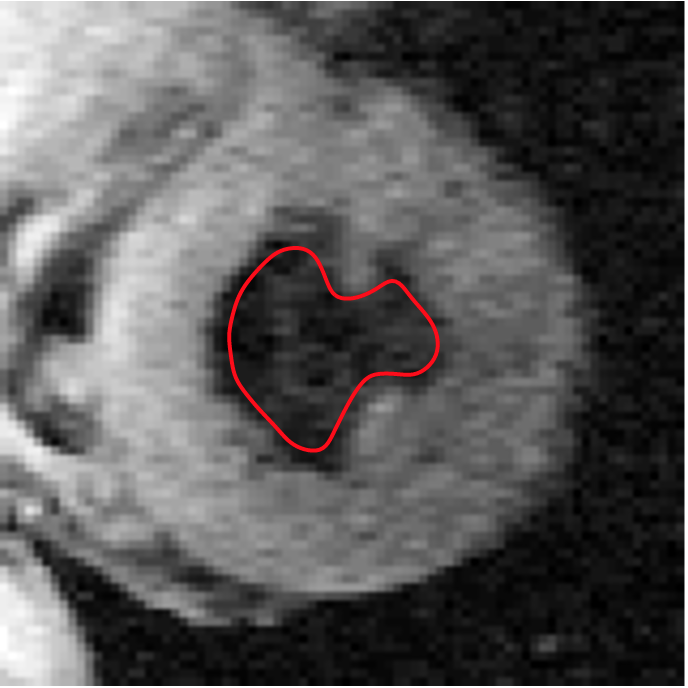
\includegraphics[width=40mm]{img/b0_0}}
\subfigure[$\beta=0.0001$]{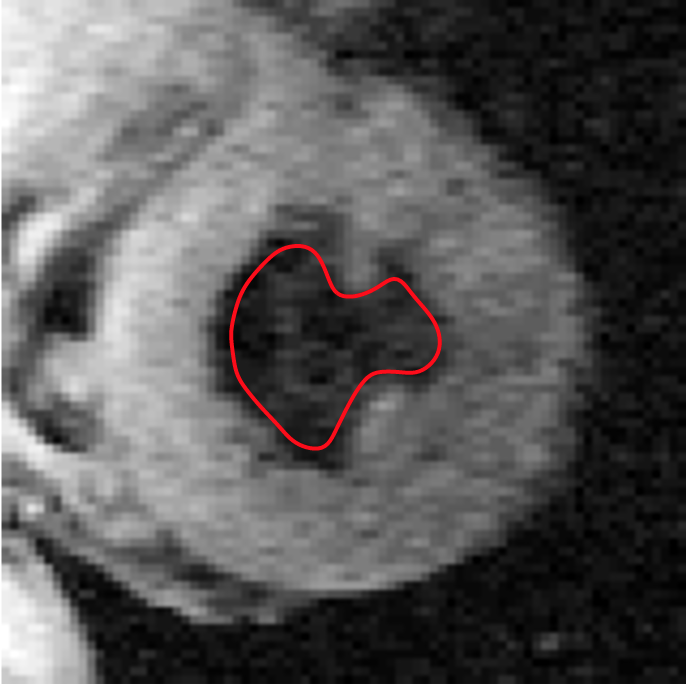
\includegraphics[width=40mm]{img/b0_0001}}
\subfigure[$\beta=0.01$]{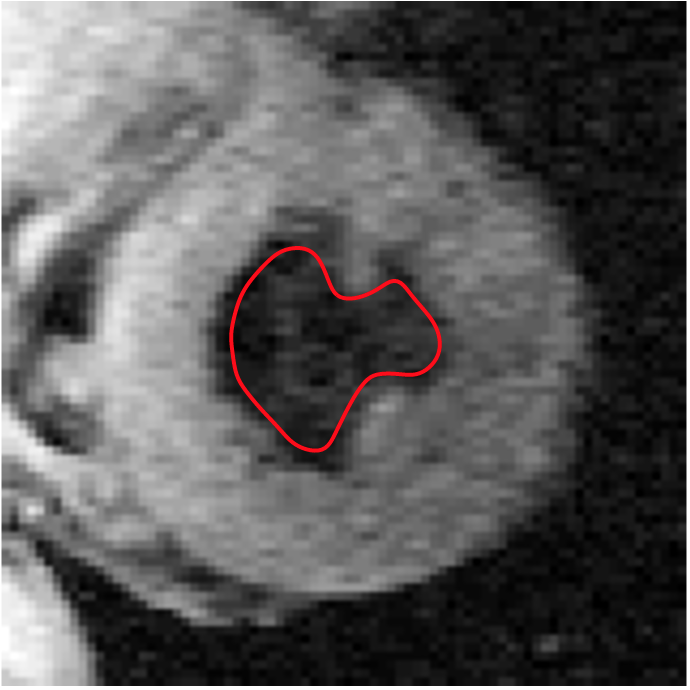
\includegraphics[width=40mm]{img/b0_01}}
\caption{Heart: tweaking the values of $ \beta $. $\beta \leq 0.01$}
\label{fig:beta_leq}
\end{figure}

Increasing $\beta$ to $0.55$ shows a more rigid shape with less defined curves. This change leads to worse results than the initial configuration. A critical value is reached for $0.65$, when the model fails to grow beyond the initial shape, see figure \ref{fig:beta_geq}. $0.01$ seems to be the optimal value for this parameter.

\begin{figure}[!hbt]
\centering   
\subfigure[$\beta=0.01$]{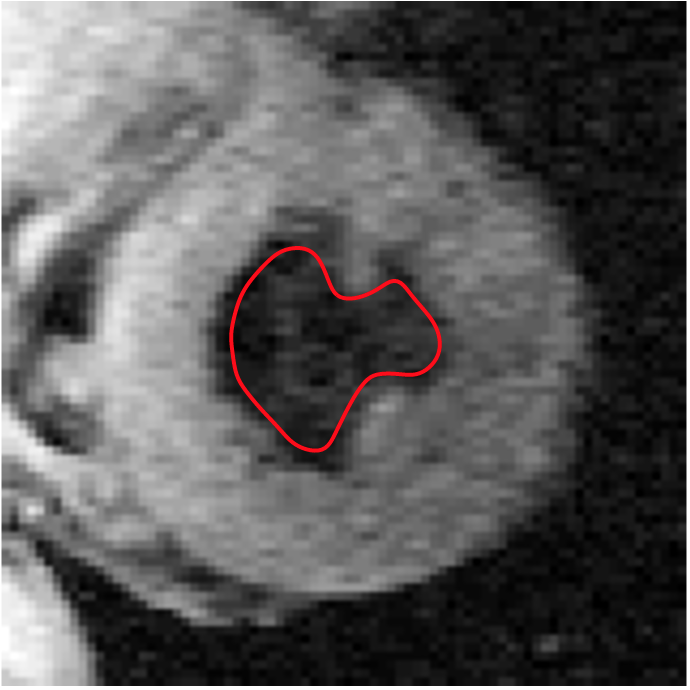
\includegraphics[width=40mm]{img/b0_01}}
\subfigure[$\beta=0.55$]{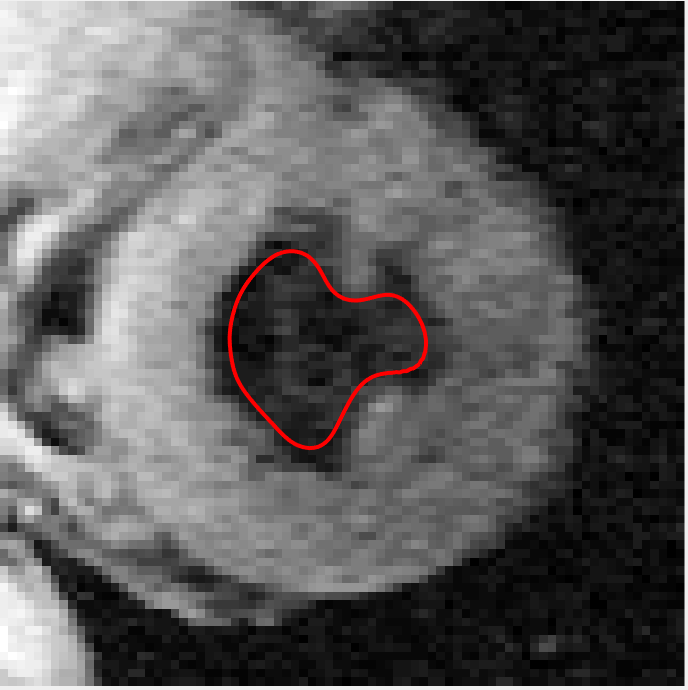
\includegraphics[width=40mm]{img/b0_55}}
\subfigure[$\beta=0.65$]{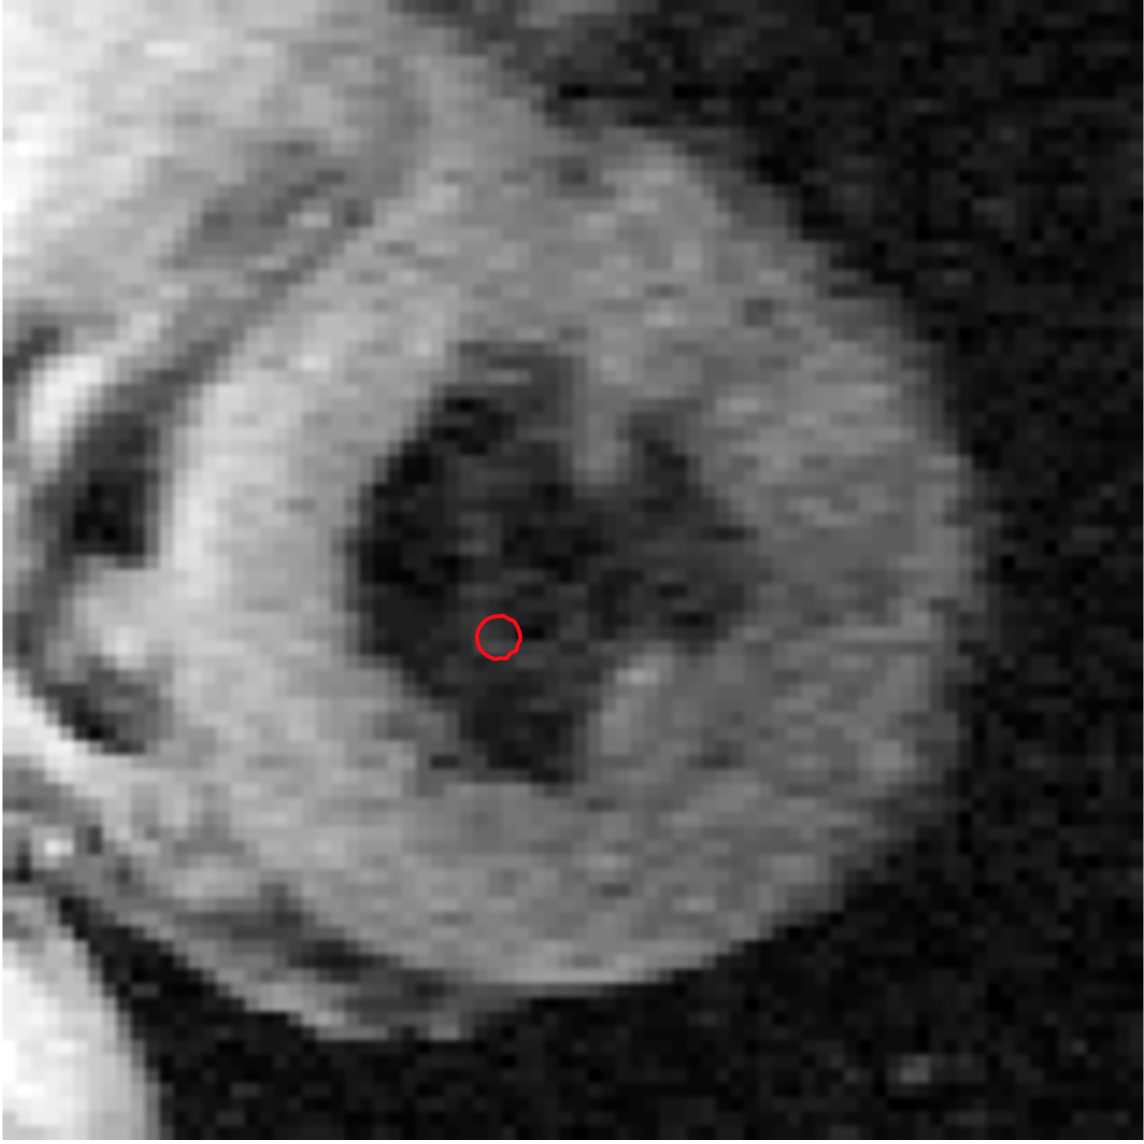
\includegraphics[width=40mm]{img/b0_65}}
\caption{Heart: tweaking the values of $ \beta $. $\beta \geq 0.01$}
\label{fig:beta_geq}
\end{figure}

\subsubsection{Kappa}

(\textbf{NOTE}: Any numerical value mentioned here actually refers to $ \kappa' $) Kappa controls the proportion of the external force which is based on the image's gradient. The higher the absolute value of kappa, the stronger the influence of the external force on the shaping of the model (as opposed to the balloon force, see section \ref{sub:forces}). For high values of kappa, the model will stop at very weak edges. Our experiments show that the initial value of $0.2$ is near optimal. When decreasing kappa to $0.18$, the shape over-extends a little on the top part where the gradient of the surrounding shape is not yet strong enough. Further decreasing to $0.16$ leads to a critical value where the model fails to stop at the relevant edges and outgrows the entire area. See figure \ref{fig:kappa_leq}.

\begin{figure}[!hbt]
\centering   
\subfigure[$\kappa=0.16$]{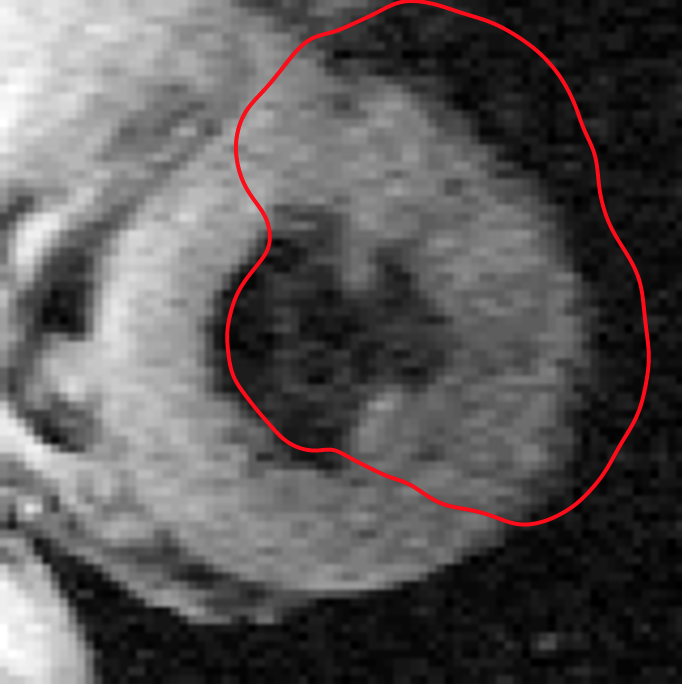
\includegraphics[width=40mm]{img/k0_16}}
\subfigure[$\kappa=0.18$]{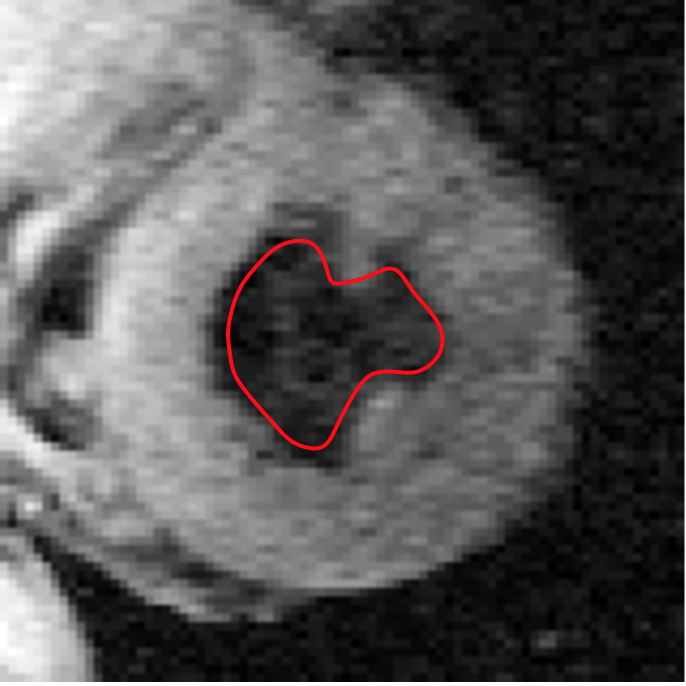
\includegraphics[width=40mm]{img/k0_18}}
\subfigure[$\kappa=0.2$]{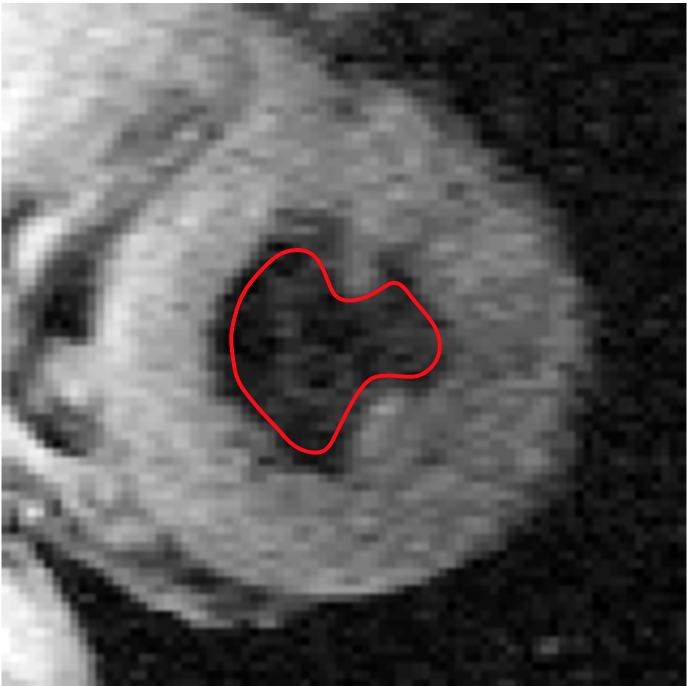
\includegraphics[width=40mm]{img/k0_2}}
\caption{Heart: tweaking the values of $ \kappa $. $\kappa \leq 0.2$}
\label{fig:kappa_leq}
\end{figure}

As figure \ref{fig:kappa_geq} shows, increasing kappa above the initial value of $0.2$ decreases segmentation quality. The external force is too strong, so small gradients that are related to noise and not the actual edge of the heart get weighted enough to stop the model from growing. When setting kappa to $1000$ the shape fails entirely to segment the shape of the heart and follows noisy gradients towards a triangular shape, see figure \ref{fig:kappa_geq} (c).

\begin{figure}[!hbt]
\centering   
\subfigure[$\kappa=0.2$]{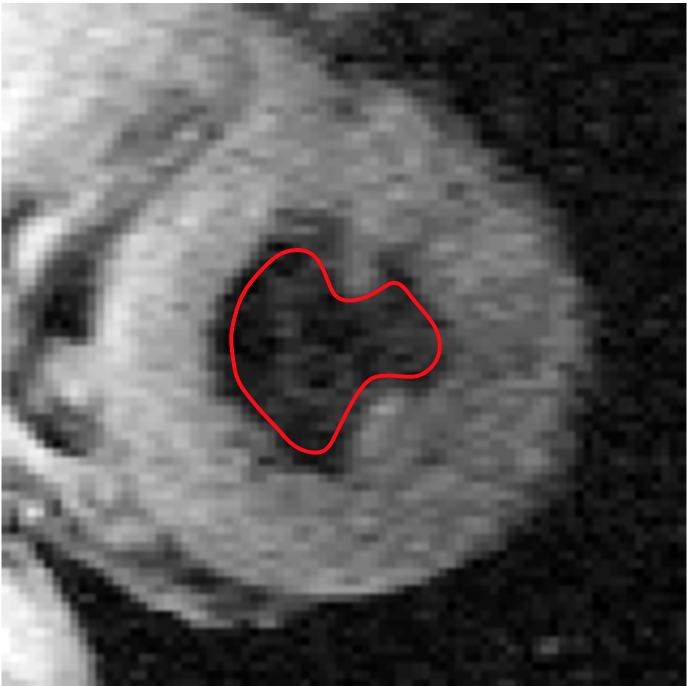
\includegraphics[width=40mm]{img/k0_2}}
\subfigure[$\kappa=0.4$]{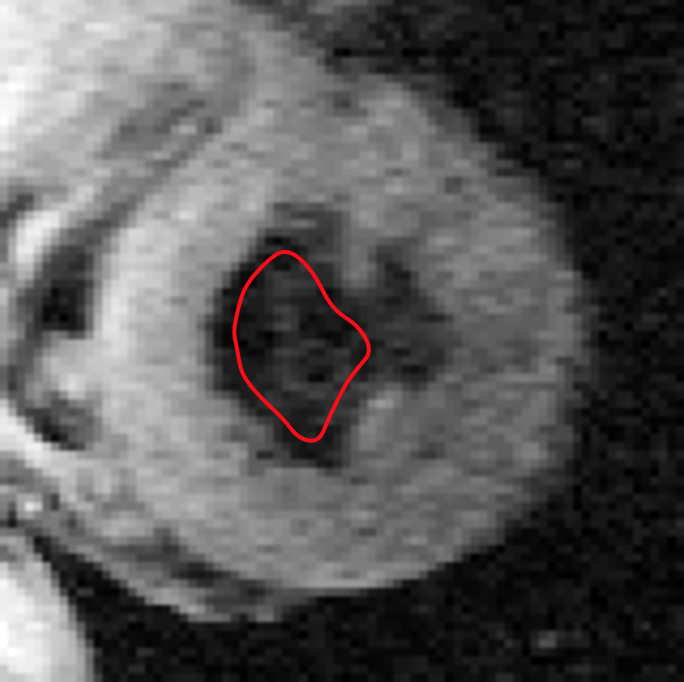
\includegraphics[width=40mm]{img/k0_4}}
\subfigure[$\kappa=1000$]{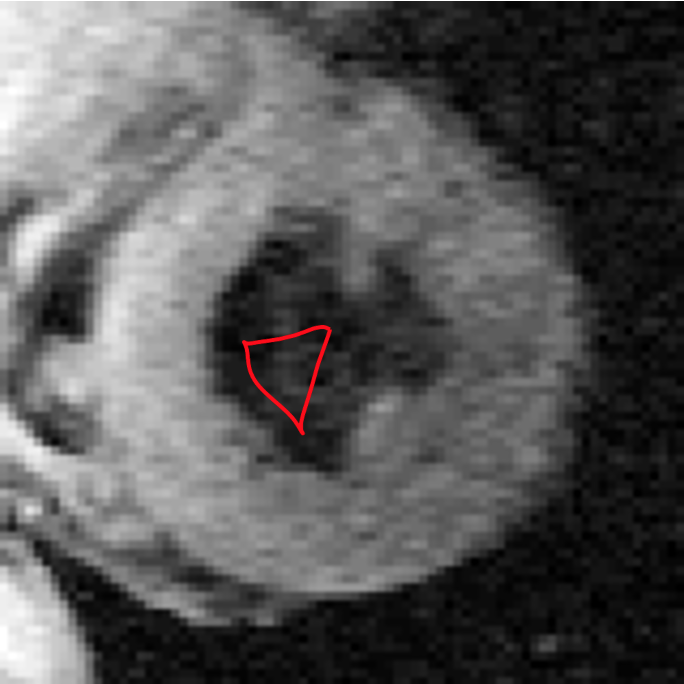
\includegraphics[width=40mm]{img/k1000}}
\caption{Heart: tweaking the values of $ \kappa $. $\kappa \geq 0.2$}
\label{fig:kappa_geq}
\end{figure}

\subsubsection{Lambda}

Lambda defines the weight of the balloon force, as opposed to the external force being controlled by the kappa parameter. A high value of lambda corresponds to a strong balloon force. Our experiments show that when decreasing lambda to $0.02$, a critical value is reached where the model fails to grow, since the internal energy trying to keep the points close together is stronger. This can be observed in figure \ref{fig:lambda_leq}. The values of lambda are positive since our initial shape lies within the shape we want to segment and thus our model needs to expand. For negative lambdas, the model would contract instead.

\begin{figure}[!hbt]
\centering   
\subfigure[$\lambda=0.02$]{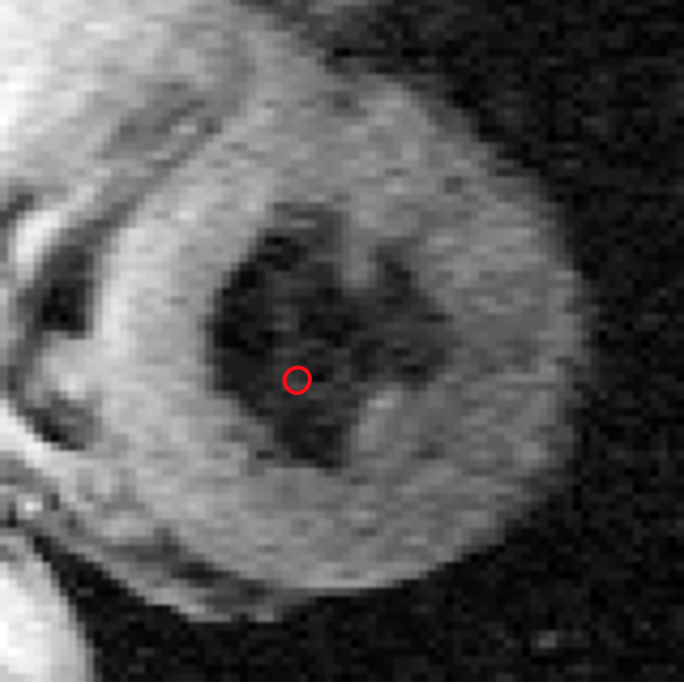
\includegraphics[width=40mm]{img/l0_02}}
\subfigure[$\lambda=0.04$]{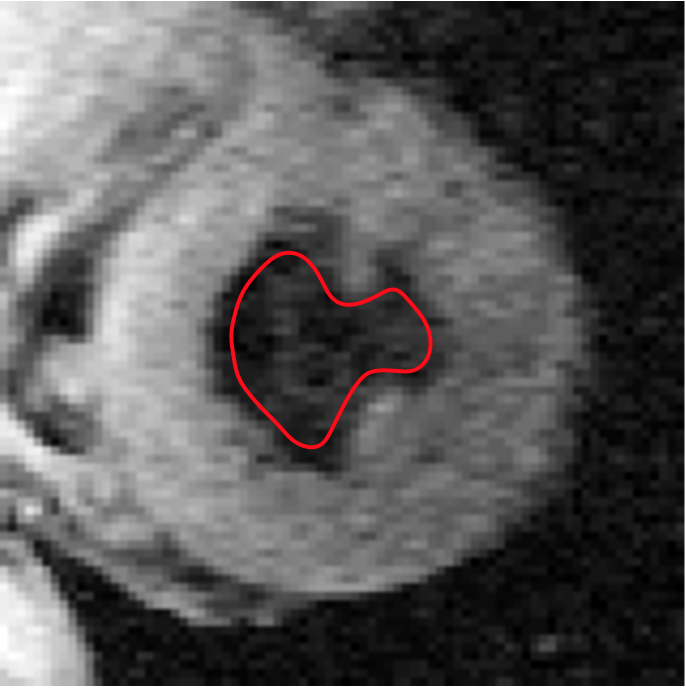
\includegraphics[width=40mm]{img/l0_04}}
\subfigure[$\lambda=0.05$]{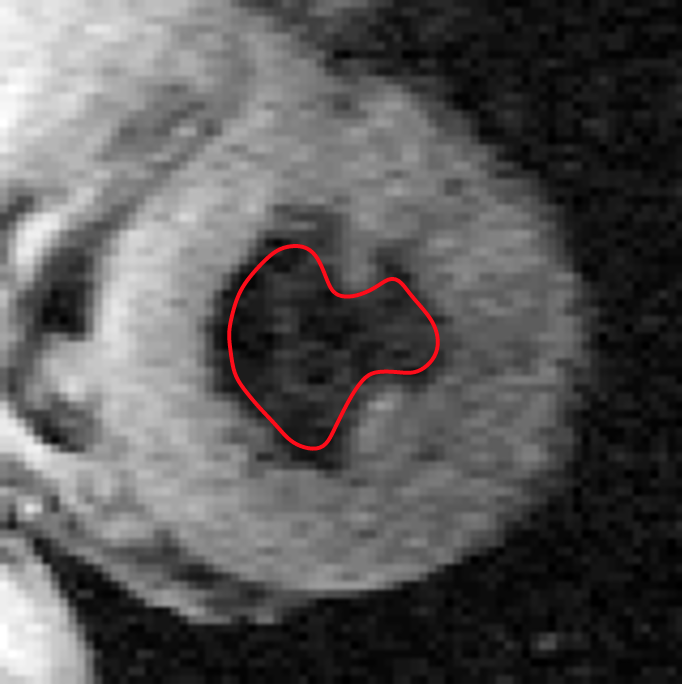
\includegraphics[width=40mm]{img/l0_05}}
\caption{Heart: tweaking the values of $ \lambda $. $\lambda \leq 0.05$}
\label{fig:lambda_leq}
\end{figure}

As figure \ref{fig:lambda_geq} shows, even just slightly increasing lambda to $0.055$ already worsens the result - the balloon force is weighted too strongly. For a value of $0.06$, the model expands to much and outgrows the wanted shape. Thus, the optimal value seems to be close to $0.05$.

\begin{figure}[!hbt]
\centering   
\subfigure[$\lambda=0.05$]{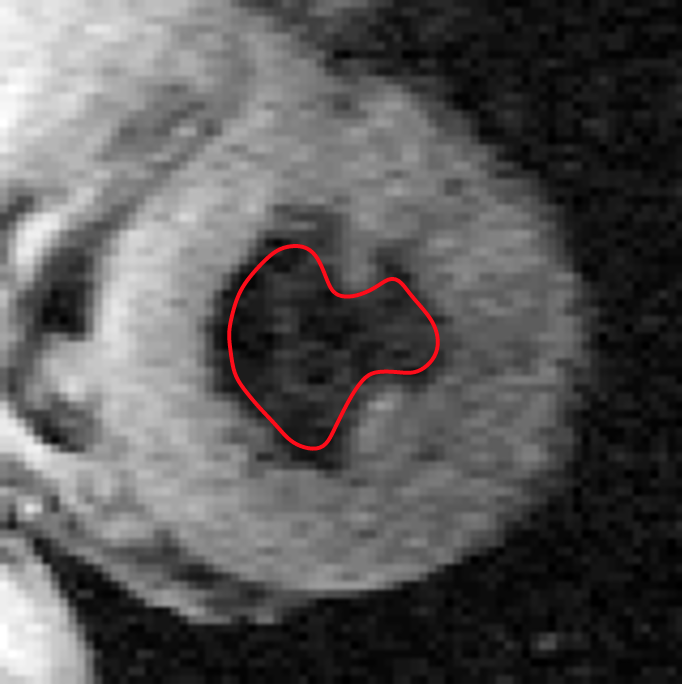
\includegraphics[width=40mm]{img/l0_05}}
\subfigure[$\lambda=0.055$]{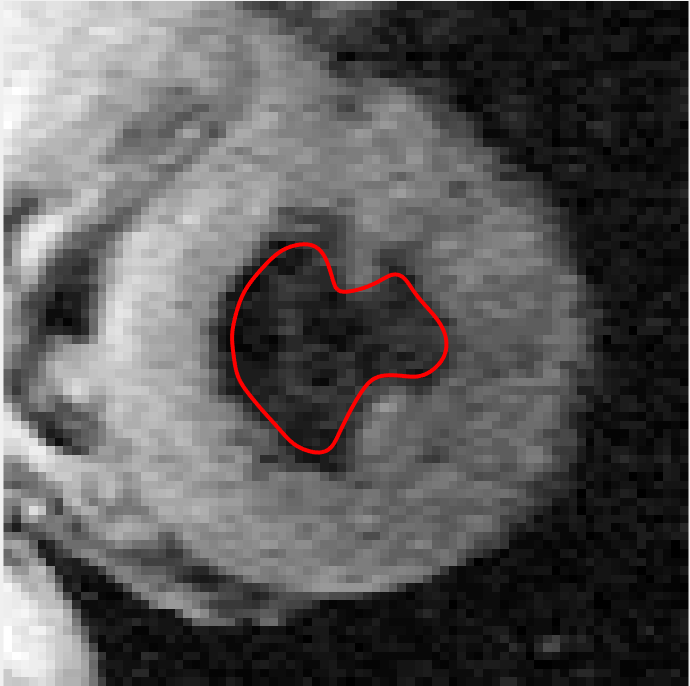
\includegraphics[width=40mm]{img/l0_055}}
\subfigure[$\lambda=0.06$]{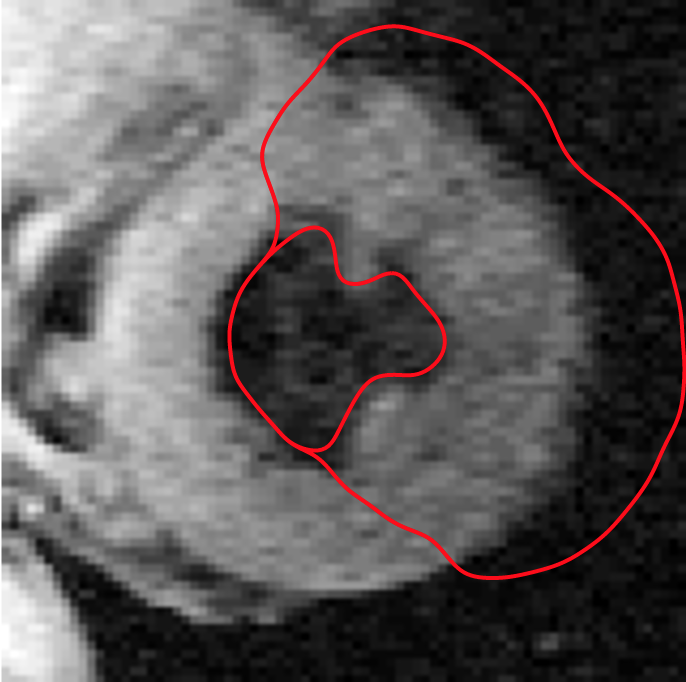
\includegraphics[width=40mm]{img/l0_06}}
\caption{Heart: tweaking the values of $ \lambda $. $\lambda \geq 0.05$}
\label{fig:lambda_geq}
\end{figure}

\subsection{Maxstep}

Increasing maxstep did not lead to any changes of the segmentation's results in our experiments. However, as figure \ref{fig:max_leq} shows, when choosing a very small value such as $0.001$, a critical value is reached where the model fails to grow.

\begin{figure}[!hbt]
\centering   
\subfigure[$maxstep=0.001$]{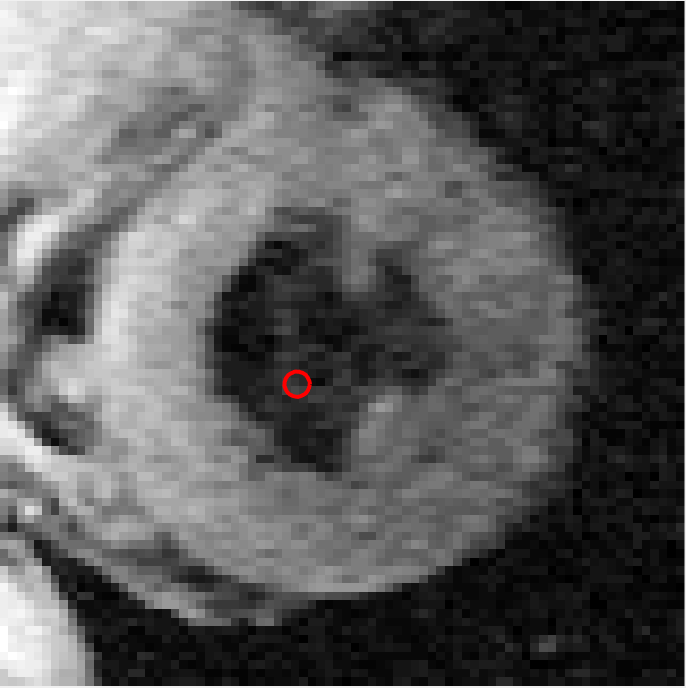
\includegraphics[width=40mm]{img/m0_001}}
\subfigure[$maxstep=0.01$]{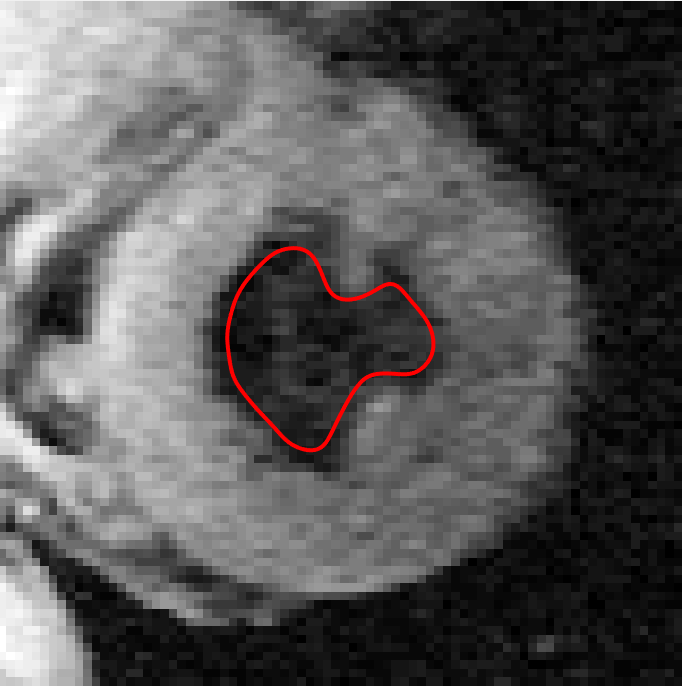
\includegraphics[width=40mm]{img/m0_01}}
\subfigure[$maxstep=0.4$]{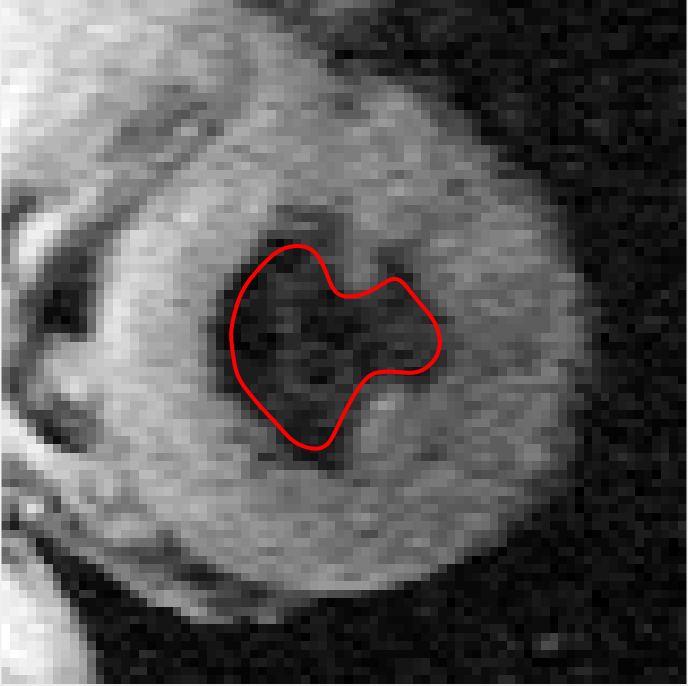
\includegraphics[width=40mm]{img/m0_4}}
\caption{Heart: tweaking the values of maxstep. $maxstep \leq 0.4$}
\label{fig:max_leq}
\end{figure}

\subsection{Forces of the Segmentation}
\label{sub:forces}

There are different forces at work that control the growing of the model. The curves are drawn toward edges by the potential force, defined as the negative gradient of a potential function, in this case the gray scale image smoothed with a Gaussian kernel. Together with the balloon force, that pushes the model to expand (for positive $\lambda$) or contract (for negative $\lambda$), the potential force contributes to the external force. At the same time, internal forces define the properties of the model: trying to keep the points of the model close together (elasticity) and avoiding bending too much (rigidity). 

We can visualize the potential force field of the heart image for both the x and y dimensions in figure
\ref{fig:ffhx}

\begin{figure}[!hbt]
\centering   
\subfigure[x dimension]{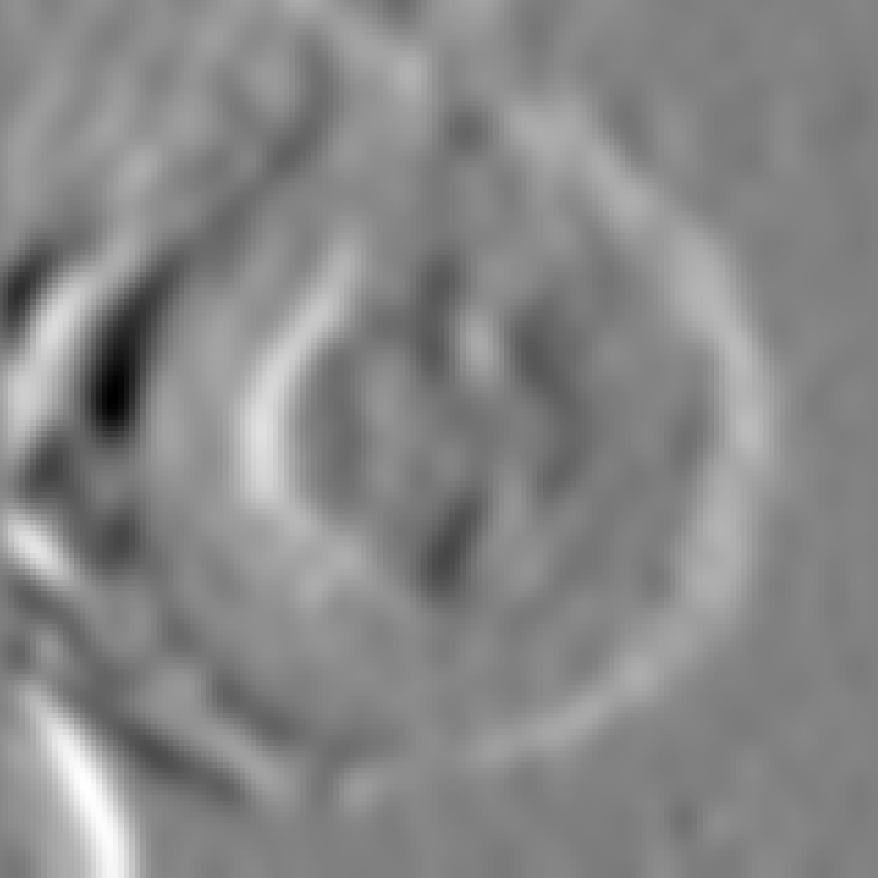
\includegraphics[width=60mm]{img/forcef_heart_x.png}}
\subfigure[y dimension]{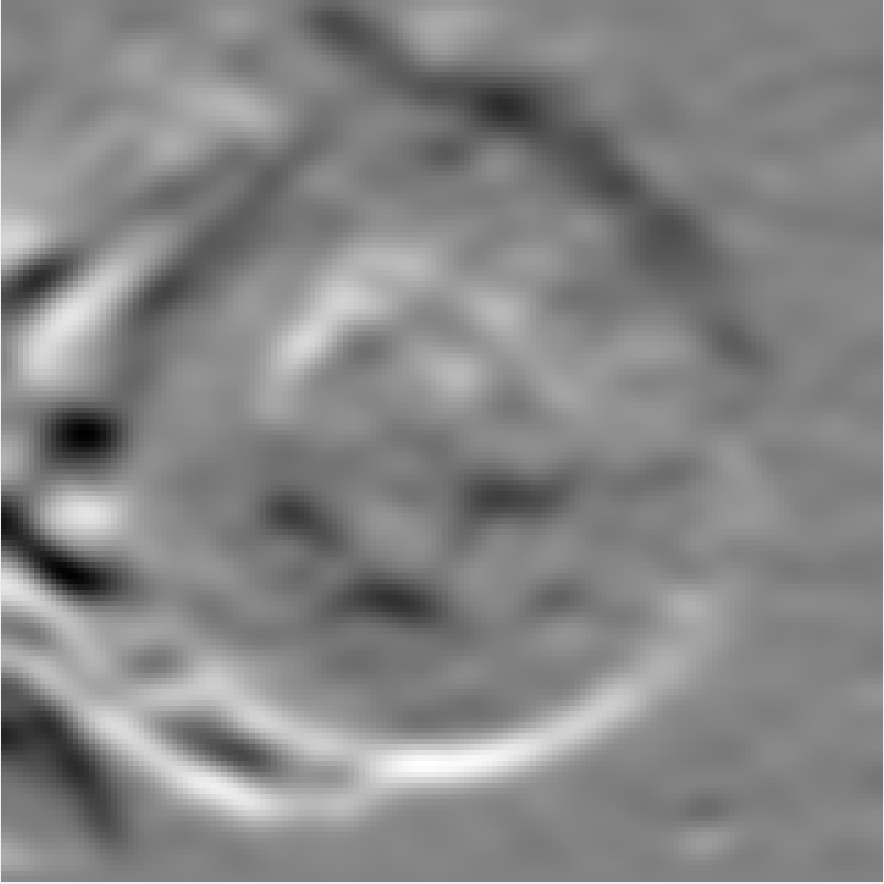
\includegraphics[width=60mm]{img/forcef_heart_y.png}}
\caption{Force Field of Heart Segmentation}
\label{fig:ffhx}
\end{figure}

As said before, the external force is a combination of the potential force visualized in figure \ref{fig:ffhx} and the balloon force, and the weight of each component is controlled by means of the
$\kappa$ and $\lambda$ parameters.
